\section{Постановка задачи}

Постановка задачи:

\begin{enumerate}
    \item Установить и настроить IBM LSF;
    \item Поддержать API для LSF в серверной части Scheduler;
    \item Поддержать команды, направляемы напрямую из Scheduler на кластер;
    \item Протестировать.
\end{enumerate}

На блок-схеме \ref{fig:block-scheme} изображены отношения между элементами. Каждый элемент не знает о элементах за элементом, с которым он связан. Каждый элемент служит абстракцией.

\begin{figure}[h]
    \centering
    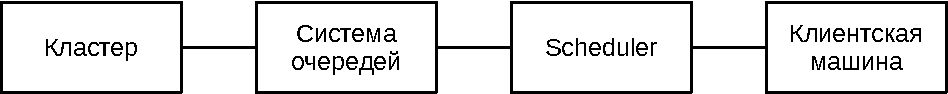
\includegraphics{scheme.pdf}
    \caption{Блок-схема}
    \label{fig:block-scheme}
\end{figure}

\clearpage
